\documentclass{beamer}

\usepackage{default}
\usepackage[portuguese]{babel}
\usepackage[utf8]{inputenc}
\usepackage{graphicx}
\usepackage{hyperref}
\usepackage{mdwlist}
\usepackage{textcomp}
\usepackage{graphicx}
\usetheme{Antibes}


\title{Introdução à simulação de circuitos com o \textit{LTspice IV}}
\author{Renan Birck Pinheiro}
\institute{Universidade Federal de Santa Maria}

\begin{document}

\begin{frame}
\titlepage
\end{frame}

\begin{frame} % slide introdução
\frametitle{Introdução}
\begin{itemize}
\item{Por que simular circuitos?}
\begin{itemize}
\pause
\item{Complexidade do projeto de novos circuitos}
\pause
\item{Reduzir custos de prototipagem}
\pause
\item{Simplificar o processo de projeto}
\pause
\item{entre outros.}
\end{itemize}
\end{itemize}
\end{frame} % slide introdução

\begin{frame} % slide SPICE
\frametitle{SPICE}
\begin{itemize}
\item{\textbf{S}imulation \textbf{P}rogram \textbf{W}ith \textbf{I}ntegrated \textbf{C}ircuit \textbf{E}mphasis - Ferramenta de Simulação com Ênfase em Circuitos Integrados}
\item{\textbf{Primeiras versões}: FORTRAN, anos 70, grandes computadores, modo texto}
\item{\textbf{SPICE 2}: linguagem C, anos 80/90, computadores de pequeno/médio porte, interface gráfica simples}
\item{\textbf{Versões atuais}: C/C++, computadores pessoais, interface gráfica avançada, desenho de circuitos}
\pause
\item{\textbf{Vários fabricantes} pegaram o código e fizeram suas próprias versões adicionando recursos}
\begin{itemize}
\item{\textbf{Motivação}: atender interesses específicos de indústrias: microeletrônica, RF etc...}
\item{Assim, temos hoje diversos simuladores: PSpice, HSpice, LTspice, Spectre, Proteus entre outros}
\end{itemize}
\end{itemize}
\end{frame} % slide SPICE

\begin{frame}
Vantagens:
\begin{itemize}
\item{\textbf{Projeto}} mais rápido, podem-se testar diversos componentes antes da compra.
\item{Realizar \textbf{medidas}} que muitas vezes são difíceis de fazer na bancada.
\item{\textbf{Projeto iterativo}}, usando métodos de otimização para atender requisitos.
\end{itemize}

\end{frame}

\begin{frame}
Desvantagens:
\begin{itemize}
\item{\textbf{Não substitui prototipagem:} os modelos são aproximados, não levam efeitos térmicos ou as componentes parasitas da placa}
\item{\textbf{Necessidade} de modelos para os componentes}
\item{O simulador deverá \textbf{suportar} as tecnologias usadas}


\item{Em geral: \textbf{lixo entra, lixo sai}. Os resultados das simulações são tão bons quanto os modelos e o projeto do circuito forem.}
\end{itemize}
\end{frame}

\begin{frame}

\begin{figure}[htb]
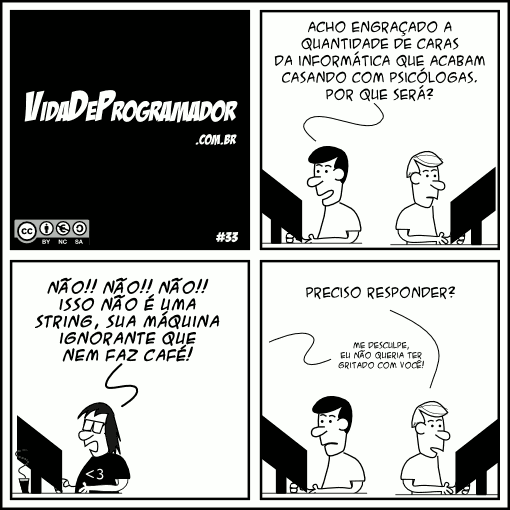
\includegraphics[width=170px]{images/tirinha33}
\caption{O simulador é uma "máquina ignorante" que só faz o que ele é mandado. Pena que ele não faz café}
\label{fig:lixoentrasai}
\end{figure}

\end{frame}

\begin{frame}
\frametitle{Obtendo e instalando o LTspice}
\begin{itemize}
\item \url{http://www.linear.com/ltspice} $\rightarrow$ \textit{Download LTspice IV}
\item Proceder com a instalação, será criado um ícone na área de trabalho.
\end{itemize}
\end{frame}

\begin{frame}
\frametitle{Desenhando um circuito}
\end{frame}

\begin{frame}
\frametitle{Componentes}
\begin{itemize}
\item {Acessíveis pelo teclado:} Resistor (R), capacitor (C), indutor (L), diodo (D)
\item {No menu de componentes (aperte F2)}: Fonte de tensão (\textit{Voltage}) e de corrente (\textit{Current}), transistores (\textit{npn/pnp}, \textit{njf/pjf} (FET), \textit{nmos/pmos} (MOSFET))
\end{itemize}
\end{frame}

\begin{frame}
\frametitle{Parâmetros: fontes de tensão/corrente}
Clique com o botão direito na fonte e após clique em Advanced. Aparecerá uma janela com diversas configurações possíveis para a fonte.
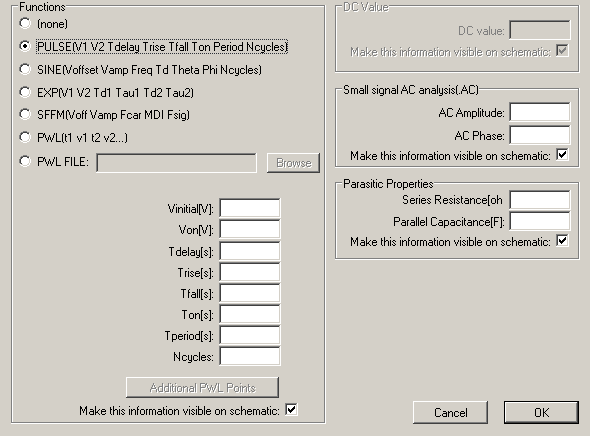
\includegraphics[width=150px]{images/paramfonte.png}
\end{frame}

\begin{frame}
\end{frame}

\begin{frame}
\frametitle{Parâmetros: resistores, capacitores e indutores}
\begin{itemize}
\item{Para capacitores e indutores, podemos definir \textbf{condições iniciais} de tensão e corrente, respectivamente...}
\item{... mas elas só serão respeitadas se marcarmos \textit{Use initial Conditions} nos parâmetros de simulação}
\end{itemize}
\end{frame}

\begin{frame}
\frametitle{Parâmetros: semicondutores}
\begin{itemize}
\item{Modelos de semicondutores contêm os parâmetros que serão usados pelas equações de dispositivos.}
\item{Normalmente esses modelos são fornecidos pelos fabricantes.}
\item{Componentes mais complexos (\textit{op-amps}, \textit{buffers} etc...) estão disponíveis na forma de subcircuitos.}
\end{itemize}
\end{frame}


\begin{frame}
\frametitle{Análise transiente}
\begin{itemize}
\item{Simulação no domínio do tempo, para circuitos lineares ou não, empregando as equações de dispositivos e as técnicas de análise de circuitos}
\end{itemize}
\end{frame}

\begin{frame}
\frametitle{Análise transiente - opções de configuração}
\begin{itemize} 
\item \textit{Stop Time}: por quanto tempo executar a simulação
\item \textit{Time to Start Saving Data}: quando começar a salvar dados?
\item \textit{Start external DC supplies at 0V}: iniciar as fontes DC em 0V; após 20 $\mu$s elas subirão ao nível especificado
\item \textit{Skip Initial Operating Point Solution}: usar as condições iniciais especificadas anteriormente (se não tiver nenhuma, ele usa 0 V), caso contrário ele tenta calcular um ponto de operação DC.
\end{itemize}
\end{frame}

\begin{frame}
\frametitle{Exemplo 1: Circuitos RC e RLC}
\end{frame}

\begin{frame}
\frametitle{Exemplo 2: Transformador}
Usamos o elemento $K$ para definir um acoplamento magnético entre dois indutores.
\end{frame}

\begin{frame}
\frametitle{Exemplo 3: Circuito a transistor}
\end{frame}


\begin{frame}
\frametitle{Análise AC}
\begin{itemize}
\item{Análise de pequenos sinais no \textbf{domínio da frequência}}
\item{Circuitos não-lineares são \textbf{linearizados} ao redor do ponto de operação}
\item{As fontes são definidas como fasores com módulo e fase}
\item{Por exemplo: Fonte definida como \texttt{AC 1 0} = $1\measuredangle 0$} 
\end{itemize}
\end{frame}

\begin{frame}
\frametitle{Análise AC - Opções de configuração}
\begin{itemize}
\item{\textit{Type of Sweep}}: seleciona se a varredura é feita por oitavas, por décadas, de forma linear ou para pontos especificados.
\begin{itemize}
\item{Oitava}: faixa de frequências de $f$ a $2 f$
\item{Década}: faixa de frequências de $f$ a $10 f$
\end{itemize}
\item{\textit{Number of Points}}: número de pontos.
\item{\textit{Start Frequency/Stop Frequency}}: frequências de início e de fim.
\end{itemize}
\end{frame}

\begin{frame}
\frametitle{Exemplo 4: Circuito com amplificador operacional}
\end{frame}

\begin{frame}
\frametitle{Análise de varredura DC}
\end{frame}

\begin{frame}
\frametitle{Exemplo 5: Curvas do diodo}
\end{frame}

\begin{frame}
\frametitle{Análise de Fourier}
\begin{itemize}
\item Permite visualizar o conteúdo harmônico de um sinal, isto é, as frequências que formam esse sinal.
\item \textbf{Sempre} especificar o parâmetro \textit{plotwinsize=0}, para desativar a compactação (que pode resultar na perda de componentes do sinal).
\end{itemize}
\end{frame}

\begin{frame}
\frametitle{Exemplo 6: Modulador AM a transistor}
\end{frame}

\begin{frame}
\frametitle{Resultados}
Da teoria de Fourier, sabemos que ao multiplicarmos um sinal de frequência $F_s$ por uma portadora de frequência $F_c$ (modulação em amplitude), obtemos as harmônicas $F_s + F_c$ e $F_s - F_c$. E isso fica visível no gráfico.
\end{frame}

\begin{frame}
\frametitle{Medição de THD com Fourier}
\begin{itemize}
\item Excita-se o circuito com um sinal senoidal naentrada, e determina-se o conteúdo harmônico da saída.
\begin{itemize}
\item Sintaxe: \texttt{.four freq-fundamental V(out)}
\item Obs.: \textbf{definir uma análise transiente antes}
\end{itemize}
\end{itemize}
\end{frame}

\begin{frame}
\frametitle{Exemplo 7: Amplificador \textit{push-pull}}
\end{frame}

\begin{frame}
\frametitle{Links de interesse}
\begin{itemize}
\item \url{http://tech.groups.yahoo.com/group/LTspice/} - grupo de usuários do LTspice
\end{itemize}
\end{frame}

\begin{frame}
{\LARGE OBRIGADO!}
\end{frame}

\begin{frame}
Contatos: \url{renan.ee.ufsm@gmail.com} \url{http://facebook.com/renanbirck} \url{http://twitter.com/renan2112}\newline

O código-fonte desses slides e os circuitos empregados estão disponíveis em \url{https://github.com/renanbirck/minicurso-2012} ou com o autor.

Crédito das tirinhas: Vida de Programador \url{http://www.vidadeprogramador.com.br}
\end{frame}
\end{document}
